\lecture{Segurança no Desenvolvimento de Sistemas}{dev}
\lecturetitle{\insertlecture}{\course}
\frame{\maketitle}

% Validação da entrada de dados

\frame{\author{}\date{}\title{Estouro de {\it buffer\/}}\maketitle}


\begin{frame}[fragile]{Estouro de {\it buffer\/}}

O estouro de {\it buffer\/} ({\it buffer overflow}) pode ocorrer em programas
escritos em C ou C++ que não fazem a verificação dos limites durante a
escrita em vetores. As funções que não fazem a verificação do tamanho
do {\it buffer\/} permitem que um vetor de tamanho arbitrário seja fornecido
ao programa. Como exemplo, temos a função {\tt gets()}, que faz parte do
padrão ANSI C, e tem como protótipo:

\begin{lstlisting}
char *gets(char *s);
\end{lstlisting}

e quando invocada, lê a partir da entrada-padrão, 
escrevendo o conteúdo lido na variável {\tt char *s}.

\end{frame}

\begin{frame}[fragile]{}

O trecho de programa a seguir mostra seu uso, onde o vetor {\tt line\/}
possui tamanho 128, porém, se o usuário fornecer como argumento um
vetor maior que 128, este será escrito na variável {\tt line}:

\begin{lstlisting}
main() {
  char line[128];
  /* ... */
  gets(line);
}
\end{lstlisting}

\end{frame}

\begin{frame}[fragile]{}

Uma solução para este problema seria usar funções que fazem a
verificação do tamanho do argumento de entrada. No lugar da função 
{\tt gets()} poderíamos usar a função {\tt fgets}, cujo protótipo é

\begin{lstlisting}
char *fgets(char *s, int size, FILE *stream);
\end{lstlisting}

e quando invocada, lê um caracter a menos que o tamanho
fornecido em {\tt size} do arquivo {\tt stream} e escreve na variável
{\tt s}.
\end{frame}


\begin{frame}[fragile]{}

O programa poderia ser reescrito usando {\tt fgets}, fornecendo o
tamanho máximo da escrita no arquivo {\tt stdin}, que é a
entrada-padrão.

\begin{lstlisting}
main() {
  char line[128];
  /* ... */
  fgets(line, 128, stdin);
}
\end{lstlisting}

\end{frame}

\begin{frame}[fragile]{}

Outra função da biblioteca-padrão C que possui problemas pela não verificação 
do limite para a escrita é {\tt strcpy}, cujo protótipo é

\begin{lstlisting}
char *strcpy(char *dest, const char *src);
\end{lstlisting}

e quando invocada, copia o conteúdo da variável {\tt src}
para a variável {\tt dest}. Como não há verificação de tamanho para a
cópia, qualquer variável fornecida será copiada até que seja
encontrado o caracter nulo {\tt `$\backslash 0$'}.

\end{frame}



\begin{frame}[fragile]{}

É altamente recomendado o uso da função {\tt strncpy()}, cujo 
protótipo é

\begin{lstlisting}
char *strncpy(char *dest, const char *src, size_t n);
\end{lstlisting}

e quando invocada, copia até {\tt n} caracteres da variável {\tt src} para
{\tt dest}. Deste modo, mesmo que seja fornecido um vetor de tamanho
grande para {\tt src}, apenas {\tt n} caracteres serão copiados.

\end{frame}

\begin{frame}[fragile]{}

Um dos principais problemas do estouro de {\tt buffer} é que o atacante,
após a ocorrência, pode assumir o controle do fluxo de execução do
programa, o que pode comprometer a integridade, confidencialidade e
disponibilidade das informações existentes nos meios de armazenamento
acessados a partir máquinas atacadas.

\end{frame}

\begin{frame}[fragile]{}\small

A frequência com que ocorre erros de gerenciamento de memória fez com
que os projetistas das linguagens mais recentes embutissem na
linguagem formas de minimizar a possibilidade de erro. Há duas
formas utilizadas:

\begin{enumerate}
\item Coletor de lixo: o binário de execução ou máquina virtual da
linguagem de programação fica responsável pela tarefa de alocar e
liberar espaço na memória, livrando o programador desta tarefa. Linguagens
como
 \href{https://docs.microsoft.com/pt-br/dotnet/csharp/programming-guide/}{C\#},
 \href{http://lisp-lang.org/}{Common Lisp}
 \href{https://golang.org/}{Go}, \href{https://www.haskell.org/}{Haskell},
 \href{https://www.java.com/en/}{Java} e \href{http://www.swi-prolog.org/}{Prolog}
 implementam este mecanismo.
 \pause
\item Política de acesso: o uso das variáveis do programa obedece à
   políticas que buscam garantir a segurança no gerenciamento
   de memória, mesmo havendo concorrência.
   
   \href{https://www.rust-lang.org/pt-BR/}{Rust} é a principal linguagem
   a implementar este mecanismo através das abstrações de {\tt borrowing\/}
   e {\it ownership\/}.
\end{enumerate}

\end{frame}

\begin{frame}{}

Mais informações sobre estouro de {\it buffer} podem ser encontradas
no livro ``Expert C Programming: Deep C Secrets'' de Peter van der
Linden. Este livro de 1994 continua sendo um referência para quem
deseja se aprofundar na linguagem C. O artigo
\href{http://insecure.org/stf/smashstack.html}{``Smashing The Stack For Fun And Profit''}
por Aleph One também é uma boa referência, com instruções em linguagem
{\it assembly\/} que demonstram de forma mais aprofundada como ocorre o
estouro de {\it buffer\/}.

\end{frame}

\frame{\author{}\date{}\title{\it Cross-site scripting\/}\maketitle}

\begin{frame}{}
O {\it cross-site scripting\/} (XSS) é um ataque de injeção de código que
explora a execução de código JavaScript no navegador do usuário.  A
Figure mostra a injeção do código JavaScript
{\tt <script>alert(`xss a vista')</script>} na área de texto de um formulário
HTML. Este formulário é processado por um script PHP que não trata ou
valida os caracteres entrados. 

\only<1>{
\begin{figure}
  \centering
  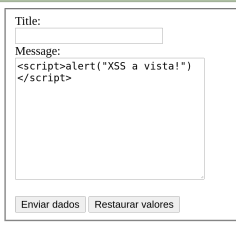
\includegraphics[scale=.5]{img/xss-snd.png}

  \caption{Envio de JavaScript usando formulário.}
\end{figure}
}

\only<2>{
  A consequência é mostrada na Figura 
  com a execução do código JavaScript.
  
\begin{figure}
  \centering
  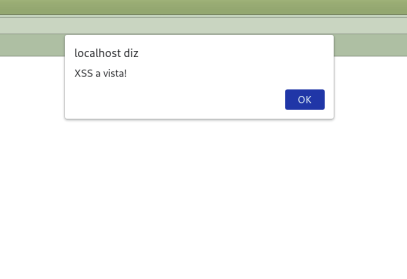
\includegraphics[scale=.5]{img/xss-rsp.png}

  \caption{Resposta do formulário após o envio do JavaScript.}
\end{figure}
}
\end{frame}

\begin{frame}[fragile]{}

O navegador Google Chrome tem um filtro chamado XSS {\it Auditor\/} que
tenta mitigar a possibilidade deste tipo de ataque bloqueando os
ataques mais comuns. Para abrir o Chrome com o filtro desabilitado,
execute:

\begin{lstlisting}[language=bash]
 google-chrome --disable-xss-auditor
\end{lstlisting}

\end{frame}

\begin{frame}{}{Envio de Javascript sem validação da entrada}

Dentre algumas das possibilidades de uso da injeção de código, podemos
listar:

\begin{itemize}
\item Roubo de {\it cookie\/}: usando a propriedade JavaScript {\tt document.cookie},
  o atacante pode obter informações dos cookies no
  navegador da vítima, enviar para seu próprio servidor e extrair
  informações sensíveis, como ID (identifição) de sessões.\pause
\item Captura de teclado: o atacante pode capturar os eventos de
  teclado usando {\tt addEventListener}, e enviar as informações
  sensíveis, como senhas e número de cartão de crédito, para seu
  servidor.\pause
\item {\it Phishing\/}: o atacante pode manipular o DOM da página e
  inserir no atributo {\it action\/} do formulário um script de seu
  servidor, enganando a vítima com a requisição de informações
  sensíveis.
\end{itemize}

\end{frame}

\begin{frame}{}

\only<1>{
      O problema pode ser corrigido tratando os caracteres de entrada,
    codificando-os de forma que não sejam interpretados pelo navegador.  A
  Figura mostra o formulário corrigido, onde os
  caracteres da área de texto são passados para a função PHP
  \href{http://php.net/manual/pt_BR/function.htmlentities.php}{\tt htmlentities()}
  
  \begin{figure}
    \centering
    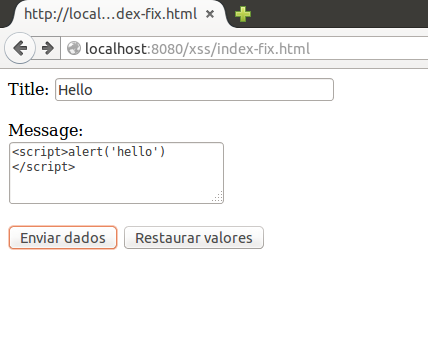
\includegraphics[scale=.5]{img/xss-fix-snd.png}
    \caption{Envio de JavaScript usando formulário.}
  \end{figure}
}

\only<2>{
  \href{http://php.net/manual/pt_BR/function.htmlentities.php}{\tt htmlentities()}
  retorna como entidade HTML, não sendo mais interpretado pelo
 navegador como mostrado na Figura.
 
 \begin{figure}
  \centering
  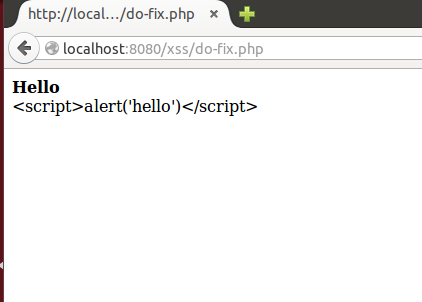
\includegraphics[scale=.5]{img/xss-fix-rsp.png}
  \caption{Resposta do formulário após o envio do JavaScript.}
 \end{figure}
}

\end{frame}

\begin{frame}{}{Envio de Javascript com tratamento da entrada}

Mais informações sobre o XSS podem ser encontradas no site
\href{http://excess-xss.com}{excess-xss.com}, criado por Jakob Kallin e Irene
Lobo Valbuena.

\end{frame}

\frame{\author{}\date{}\title{Injeção de SQL}\maketitle}

\begin{frame}[fragile]{}{Envio de SQL sem tratamento da entrada}

O ataque de injeção de SQL explora o processamento dos catacteres entrados pelo usuário pelo 
 banco de dados. A <<img-sql-snd,Figura 5>> mostra um formulário que busca os dados inseridos 
em um banco de dados PostgreSQL usando PHP. A consulta SQL feita é a seguinte:

{\small
\begin{verbatim}
pg_query($conn, "SELECT * FROM login WHERE username='" . 
  $_POST["username"]  . "' AND password='" . 
  $_POST["password"] . "'");
\end{verbatim}
}

onde {\tt \$\_POST[``username'']} contém os caracteres
inseridos no campo "Username" e {\tt \$\_POST[``password´´]} os
caracteres inseridos no campo "Password" que corresponderia à senha
do usuário.

\end{frame}

\begin{frame}[fragile]{}

Se forem fornecidos os valores {\tt alice} e {\tt alice123} para os
campos ``Username'' e ``Password'', respectivamente, a consulta no
banco de dados torna-se

\begin{lstlisting}[language=SQL]
SELECT * FROM login WHERE 
  username='alice' AND password='alice123';
\end{lstlisting}

\end{frame}

\begin{frame}{}

  Se os valores existirem na tabela {\tt login} no banco de dados, o
script PHP retorna a mensagem de sucesso, caso contrário, significa
que o usuário não está cadastrado, ou digitou a senha incorretamente,
e o script PHP retorna a mensagem de falha.
\end{frame}

\begin{frame}[fragile]{}

Se injetarmos os caracteres {\tt ` OR 1=1;--} no campo ``Username'',

\begin{lstlisting}[language=SQL]
SELECT * FROM login WHERE username='' OR 1=1;-- AND password=''
\end{lstlisting}

esta consulta será interpretados da seguinte forma pelo banco de dados
PostgreSQL:

\begin{enumerate}
\item O apóstrofo ` fecha o primeiro apóstrofo após {\tt username='},
  eliminando erro de sintaxe por string não fechada;
\item O operador {\tt OR} faz com que se uma das condições que o
  circundam for verdadeira, a expressão seja verdadeira;\pause
\item A expressão {\tt 1=1} sempre é verdadeira, tornando toda a
  avaliação até o momento verdadeira;
\item O ponto e vírgula {\tt ;} encerra a consulta;\pause
\item O comentário {\tt --} faz o analisador de consultas ignorar os
  caracteres restantes, tornando a consulta sempre bem sucedida.
\end{enumerate}
\end{frame}

\begin{frame}{}
  
  \begin{figure}
    \centering
    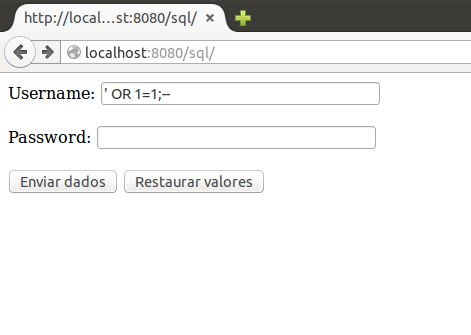
\includegraphics[scale=.5]{img/sql-snd.png}
    \caption{Envio de código SQL usando formulário.}
  \end{figure}
\end{frame}

\begin{frame}{}

  \begin{figure}
    \centering
    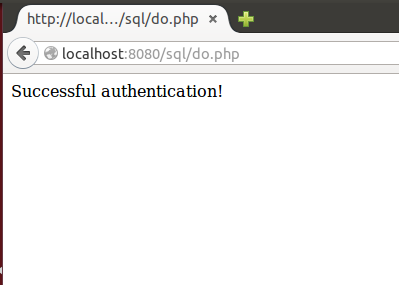
\includegraphics[scale=.5]{img/sql-rsp.png}
    \caption{Resposta do formulário após o envio do código.}
  \end{figure}
\end{frame}

\begin{frame}[fragile]{}{Envio de SQL com tratamento da entrada}

Apesar de ter sido utilizado o banco de dados PostgreSQL como exemplo,
o mesmo princípio é válido para outros bancos de dados.
Uma possível solução para o problema seria reduzir os efeitos da
concatenação de caracteres à expressão SQL original, as consultas
preparadas ({\it prepared statements}) podem ser utilizadas, como
demonstra o código PHP a seguir:

{\small
\begin{verbatim}
$res0 = pg_prepare($conn, "auth", 
           "SELECT * FROM login WHERE username=$1 AND password=$2");
$res1 = pg_execute($conn, "auth",  
            array($_POST["username"], $_POST["password"]));
\end{verbatim}
}

\end{frame}

\begin{frame}[fragile]{}

Neste caso, mesmo que caracteres de controle da linguagem SQL, tais
como o apóstrofo ``''', sejam inseridos, estes já serão tratados de
acordo com o tipo de dados esperado e não serão avaliados pelo
analisador de consulta fora de sua categoria. 

\only<1>{
\begin{figure}
  \centering
  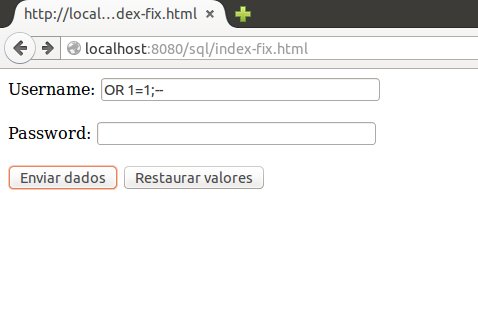
\includegraphics[scale=.5]{img/sql-fix-snd.png}
  \caption{Envio de código SQL usando formulário.}
\end{figure}  
}

\only<2>{
\begin{figure}
  \centering
  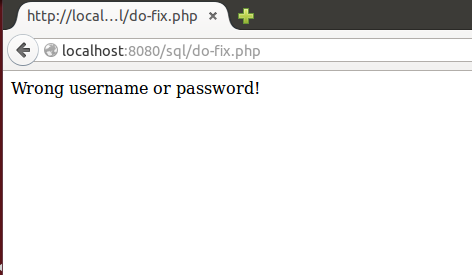
\includegraphics[scale=.5]{img/sql-fix-rsp.png}
  \caption{Resposta do formulário após o envio do código.}
  \end{figure}
}
\end{frame}

\begin{frame}{Exercícios}

  \begin{enumerate}
    \item Dê exemplo de código inseguro devido ao uso da função C `strcpy()`.
    Dê exemplo, utilizando o código, de uma entrada que poderia causar
    problemas ao rodar o programa que usa a função.

  \item Faça uma busca por falha de estouro de {\it buffer\/} em um programa conhecido
  e descreva-o, se possível, detalhando a solução adotada.

\item Descreva como o atacante poderia realizar um ataque de XSS em que
  executaria um script remoto, enviando dados do usuário ao seu
  servidor?

\item Descreva um ataque de injeção de SQL para outro banco de dados
  que não seja o PostgreSQL.
\end{enumerate}

\end{frame}